\documentclass[../main.tex]{subfiles}

\begin{document}
\chapter{Lecture 2 - 07-04-2020}

\section{Argomento}
Classification tasks\\
Semantic label space Y\\
Categorization Y finite and\\ small
Regression Y appartiene ad |R\\
How to predict labels?\\
Using the lost function $\rightarrow$ ..\\
Binary classification\\
Label space is Y = { -1, +1 }\\
Zero-one loss\\

$
\ell(y,\hat{y} = \begin{cases} 0, & \mbox{if } \hat{y} = y 
\\ 1, & 
\mbox{if }\hat{y} \neq y
\end{cases}
\\\\
FP \quad \hat{y} = 1,\quad y = -1\\
FN \quad \hat{y} = -1, \quad y = 1
$
\\\\
Losses for regression?\\
$y$, and $\hat{y} \in \barra{R}$, \\so they are numbers!\\
One example of loss is the absolute loss: absolute difference between numbers\\
\section{Loss}
\subsection{Absolute Loss}
$$\ell(y,\hat{y} = | y - \hat{y} |  \Rightarrow absolute \quad loss\\ $$
\\
\begin{figure}[h]
    \centering
    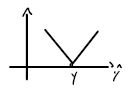
\includegraphics[width=0.4\linewidth]{../img/lez2-img1.JPG}
    \caption{Example of domain of $\knn$}
    %\label{fig:}
\end{figure}\\
\\
Some inconvenient properties:

\begin{itemize}
\item ...
\item Derivative only two values (not much informations)
\end{itemize}

\subsection{Square Loss}
$$ \ell(y,\hat{y} = ( y - \hat{y} )^2  \Rightarrow \textit{square loss}\\$$
\\
\begin{figure}[h]
    \centering
    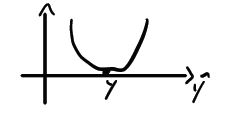
\includegraphics[width=0.4\linewidth]{../img/lez2-img2.JPG}
    \caption{Example of domain of $\knn$}
    %\label{fig:}
\end{figure}\\
\\Derivative :
\begin{itemize}
\item more informative
\item and differentible 
\end{itemize}
Real numbers as label $\rightarrow$ regression.\\
Whenever taking difference between two prediction make sense (value are numbers) then we are talking about regression problem.\\
Classification as categorization when we have small finite set.\\\\

\subsection{Example of information of square loss}

$\ell(y,\hat{y}) = ( y - \hat{y} )^2 = F(y) 
\\
F'(\hat{y}) = -2 \cdot (y-\hat{y})
$
\begin{itemize}
\item I'm under sho or over and how much
\item How much far away from the truth
\end{itemize}
$ \ell(y,\hat{y}) = | y- \hat{y}| = F(y') \cdot F'(y) = Sign (y-\hat{y} )\\\\ $
Question about the future\\
Will it rain tomorrow?\\
We have a label and this is a binary classification problem.\\
My label space will be Y = { “rain”, “no rain” }\\
We don’t get a binary prediction, we need another space called prediction space (or decision space). \\
$
Z = [0,1] \\
\hat{y} \in Z \qquad \hat{y} \textit{ is my prediction of rain tomorrow}
\\
\hat{y} = \barra{P} (y = "rain") \quad  \rightarrow \textit{my guess is tomorrow will rain (not sure)}\\\\ 
y \in Y \qquad \hat{y} \in Z \\quad \textit{How can we manage loss?}
\\
\textit{Put numbers in our space}\\
\{1,0\} \quad \textit{where 1 is rain and 0 no rain}\\\\
$
I measure how much I’m far from reality.\\
So loss behave like this and the punishment is gonna go linearly??\\
\[26..\]\\
However is pretty annoying. Sometime I prefer to punish more so i going quadratically instead of linearly.\\
There are other way to punish this.\\
I called \textbf{logarithmic loss}\\ 
We are extending a lot the range of our loss function.\\

$$
\ell(y,\hat{y}) = | y- \hat{y}| \in |0,1| \qquad \ell(y,\hat{y}) = ( y- \hat{y})^2 \in |0,1|
$$
\\
If i want to expand the punishment i use logarithmic loss\\
\\
$ \ell(y,\hat{y} = \begin{cases} ln \frac{1}{\hat{y}}, & \mbox{if } y = 1 \textit{(rain)} 
\\ ln \frac{1}{1-\hat{y}}, & 
\mbox{if } y = 0 \textit{(no rain} 
\end{cases}
\\\\
F(\hat{y}) \rightarrow \textit{can be 0 if i predict with certainty}
\\ \textit{If}\quad \hat{y} = 0.5 \qquad \ell(y, \frac{1}{2}) = ln 2 \quad \textit{constant losses in each prediction}\\\\
\lim_{\hat{y} \to 0^+}{\ell(1,\hat{y}) = + \infty} \\
\textit{We give a vanishing probability not rain but tomorrow will rain.} 
\\ \textit{So this is } +\infty \\
\lim_{\hat{y}\to 1^-} \ell(0,\hat{y}) = + \infty
\\\\ 
$
The algorithm will be punish high more the prediction is not real. Algorithm will not get 0 and 1 because for example is impossible to get a perfect prediction.\\
This loss is useful to give this information to the algorithm.\\\\
Now we talk about labels and losses\\
\subsection{labels and losses}
Data points: they have some semantic labels that denote some true about this data points and we want to predict this labels.\\
We need to define what data points are: number? Strings? File? Typically they are stored in database records \\
They can have very precise structure or more homogeneously structured \\
A data point can be viewed as a vector in some d dimensional real space. So it’s a vector of number
\\
$$
\barra{R}^d\\\\
X = (x_1,x_2 ..., x_d) \in \barra{R}^c
$$
\\
Image can be viewed as a vector of pixel values (grey scale 0-255).\\
I can use geometry to learn because point are in my Euclidean space. Data can be represented as point in Euclidean space. Images are list of pixel that are pretty much the same range and structure (from 0 to 255). It’s very natural to put them in a space.\\\\
Assume X can be a record with heterogeneous fields:\\
For example medical records, we have several values and each fields has his meaning by it’s own. (Sex, weight, height, age, zip code)\\
Each one has a different range, in some cases is numerical but something have like age ..\\
Does have any sense to see a medical record as a point since coordinates
have different meaning.\\
\textbf{Fields are not comparable.}\\
This is something that you do: when you want to solve some inference you have to decide which are the label and what is the label space and we have to encode the data points.\\\\
Data algorithm expect some homogenous interface.
In this case algorithm has to build records with different values of fields.\\
This is something that we have to pay attention too.\\
You can always each range of values in number. So ages is number, sex you
can give 0 and 1, weight number and zip code is number.\\
How ever geometry doesn’t make sense since I cannot compare this
coordinates.\\
Linear space i can sum up as vector: i can make linear combination of
vectors.\\
Inner product to measure angles! (We will see in linear classifier).\\\\
I can scramble the number of my zip code.\\
So we get problems with sex and zip code\\\\
Why do we care about geometry? I can use geometry to learn.\\
However there is more to that, geometry will carry some semantically
information that I’m going to preserve during prediction.\\
I want to encode my images as vectors in a space. Images with dog.....\\\\
PCA doesn’t work because assume we encode in linear space.\\
We hope geometry will help us to predict label correctly and sometimes i hard
to convert data into geometry point.\\
Example of comparable data: images, or documents. \\
Assume we have documents with corpus (set of documents).\\
Maybe in English and talk about different thing and different words.\\
X is a document and i want to encode X into a point fix in bidimensional
space.\\
There is a way to encode a set of documents in point in a fixed dimensional
space in such way it make sense this coordinate are comparable.\\
I can represent fields with [0,1] for Neural network for example. But they have no geometrical meaning\\

\subsection{Example TF(idf) documents encoding} 
TF encoding of docs.
\begin{enumerate}
\item Extract where all the words from docs
\item Normalize words (nouns, adjectives, verbs ...)
\item Build a dictionary of normalized words
\end{enumerate}
Doc $x = (x_1, .., x_d) $\\
I associate a coordinate for each word in a dictionary.\\
d = number of words in dictionary\\
I can decide that \\
$x_i = 1 \qquad \textit{If i-th word of dictionary occurs in doc.}\\
 x_i = 0 \qquad \textit{Else} 
$\\

$X_i\quad \textit{number of time i-th word occur in doc.}\\ $
Longer documents will have higher value of coordinates that are not zero.\\
Now i can do the TF encoding in which xi = frequency with which i-th word
occur in dictionary.\\
You cannot sum dog and cat but we are considering them frequencies so we
are summing frequency of words.\\
This encoding works well in real words.\\
I can choose different way of encoding my data and sometime i can encode a
real vector\\\\
I want
\begin{enumerate}
\item A predictor $f: X \longrightarrow Y$ (in weather $X \longrightarrow Z $
\item X is our data space (where points live)
\item $X = \barra{R}^d$ images
\item $ X = X_1 x ... x X_d$ Medical record
\item $\hat{y} = f(x) $ predictor for X
\end{enumerate}
$(x,y)$\\\\
We want to predict a label that is much closer to our label. How?\\
Loss function: so this is my setting and is called and example.\\
Data point together with label is a “example”\\
We can get collection of example making measurements or asking people. So
we can always recover the true label.\\
We want to replace this process with a predictor (so we don’t have to bored a
person).\\
y is the ground truth for x $\rightarrow$ mean reality!\\
If i want to predict stock for tomorrow, i will wait tomorrow to see the ground truth.

\end{document}